\documentclass{home_assignment}
\usepackage[acronym,nogroupskip]{glossaries}
\usepackage[sorting=none, defernumbers=true,backend=biber]{biblatex}
\addbibresource{bibliography.bib}
\makeglossaries
\newacronym{it}{IT}{Information Technology}
\newacronym{ict}{ICT}{Information and Communication Technology}
\newacronym{gdp}{GDP}{Gross Domestic Product}
\newacronym{aws}{AWS}{Amazon Web Services}
\newacronym{gcp}{GCP}{Google Cloud Platform}
\newacronym{gea}{GEA}{Government Enterprise Architecture}
\newacronym{un}{UN}{United Nations}
\newacronym{ibm}{IBM}{International Business Machines Corporation}
\newacronym{ngo}{NGO}{Non-Governmental Organization}
\newacronym{www}{WWW}{World Wide Web}
\newacronym{ntc}{NTC}{Nepal Telecom}
\newacronym{egmp}{eGMP}{e-Governance Master Plan}
\newacronym{ftth}{FTTH}{Fiber to the Home}
\newacronym{atm}{ATM}{Automated Teller Machine}
\newacronym{abbs}{ABBS}{Any Branch Banking Service}
\newacronym{isp}{ISPs}{Internet Service Providers}
\newacronym{pan}{PAN}{Permanent Account Number}
\newacronym{g2c}{G2C}{Government to Citizen}
\newacronym{g2b}{G2B}{Government to Business}
\newacronym{g2e}{G2E}{Government to Employees}
\newacronym{g2g}{G2G}{Government to Government}
\newacronym{hlcit}{HLCIT}{High Level Commission of Information and Technology}
\newacronym{dbms}{DBMS}{Database Management System}
\newacronym{nitc}{NITC}{National Information Technology Center}
\newacronym{moest}{MoEST}{Ministry of Education, Science and Technology}
\newacronym{moic}{MoIC}{Ministry of Information and Communications}
\newacronym{moga}{MoGA}{Ministry of General Administration}
\newacronym{mof}{MoF}{Ministry of Finance}
\newacronym{eta}{ETA}{Electronic Transaction Act}   
\newacronym{itu}{ITU}{International Telecommunication Union}  
\newacronym{egdi}{EGDI}{e-Government Development Index}
\newacronym{covid}{COVID-19}{Corona Virus Disease of 2019}
\usepackage{hyperref}
\newcommand\Myciteauthor[1]{\citeauthor{#1} \cite{#1}}
\begin{document}
    \titlePage{Overview of e-Governance Evolution in Nepal}{July 31, 2021}{Basanta Joshi, Ph.D.}
    \pagenumbering{roman}
    \clearpage
    \tableofcontents
    \clearpage
    \phantomsection
    \addcontentsline{toc}{section}{\bfseries{List of Figures}}
    \listoffigures
    \clearpage
    \phantomsection
    \addcontentsline{toc}{section}{\bfseries{List of Abbreviations}}
    \printglossary[type=\acronymtype,title={List of Abbreviations}]
    \clearpage
    \pagenumbering{arabic}
    \section{Introduction}
    \subsection{E-governance}
    E-governance is the use of \acrfull{ict} resources to deliver government services to the general public. This form of governance is quite necessary in the modern era since it is convenient, transparent and the most effective form to reach a larger mass of people. However, implementation of e-Governance is mostly challenging as it requires increased capabilities and expertise in the field of \acrshort{it} for policy making. The different models of e-Governance delivery can be summed up as \acrfull{g2c}, \acrfull{g2b}, \acrfull{g2e} and \acrfull{g2g}.
    \subsubsection{Challenges for E-governance in Nepal}
    \Myciteauthor{giri-egov} analyses the necessity of \acrfull{dbms} and data security in implementation of e-Governance in Nepal. The paper terms the antivirus, password, digital signature, firewall, encryption technology as data security tools and points out that an online security system should be managed attentively. \Myciteauthor{buddhacarya-lbef} points out astounding political conflicts and fluctuated political coordination as the prime barrier for e-Governance implementation. The article primarily collected the deciding data from 300 questionnaires divided evenly as online and offline, out of which 48 online and 73 offline respondents answered. \Myciteauthor{giri-practicing} highlights the challenges of civil service as a proper prospect through e-governance. The dynamic aspects of the internet can support civil services to run effectively online. However, negligence arising due to incompetence, poor implementation and mismanagement are some hinderance pointed out in the paper. The authors also point out that the issues that confine the growth of e-governance can be regulatory, legal, technical or even procedural arising from literacy, capacity building and technological growth.
    \subsection{Maturity of e-Governance}
    A set of stages or phases (from lowest to highest) that show the maturity of the e-governance implementation is called the maturity model. Some of the factors that play vital roles in the maturity of e-Governance are literacy, health, \acrfull{gdp}, political scenario. Different models have been used over the years all around the globe to rank the e-Governance maturity among one another. Various companies, states and researches propose varying maturity models, giving us a wide range of choice. \Myciteauthor{maturity} presents a comparative study among 25 such e-Government maturity models. The paper concludes with four issues that most of the maturity models use, viz. stage name, stage numbers, years and country, stage focus and stage features.
    \begin{figure}[H]
        \centering
        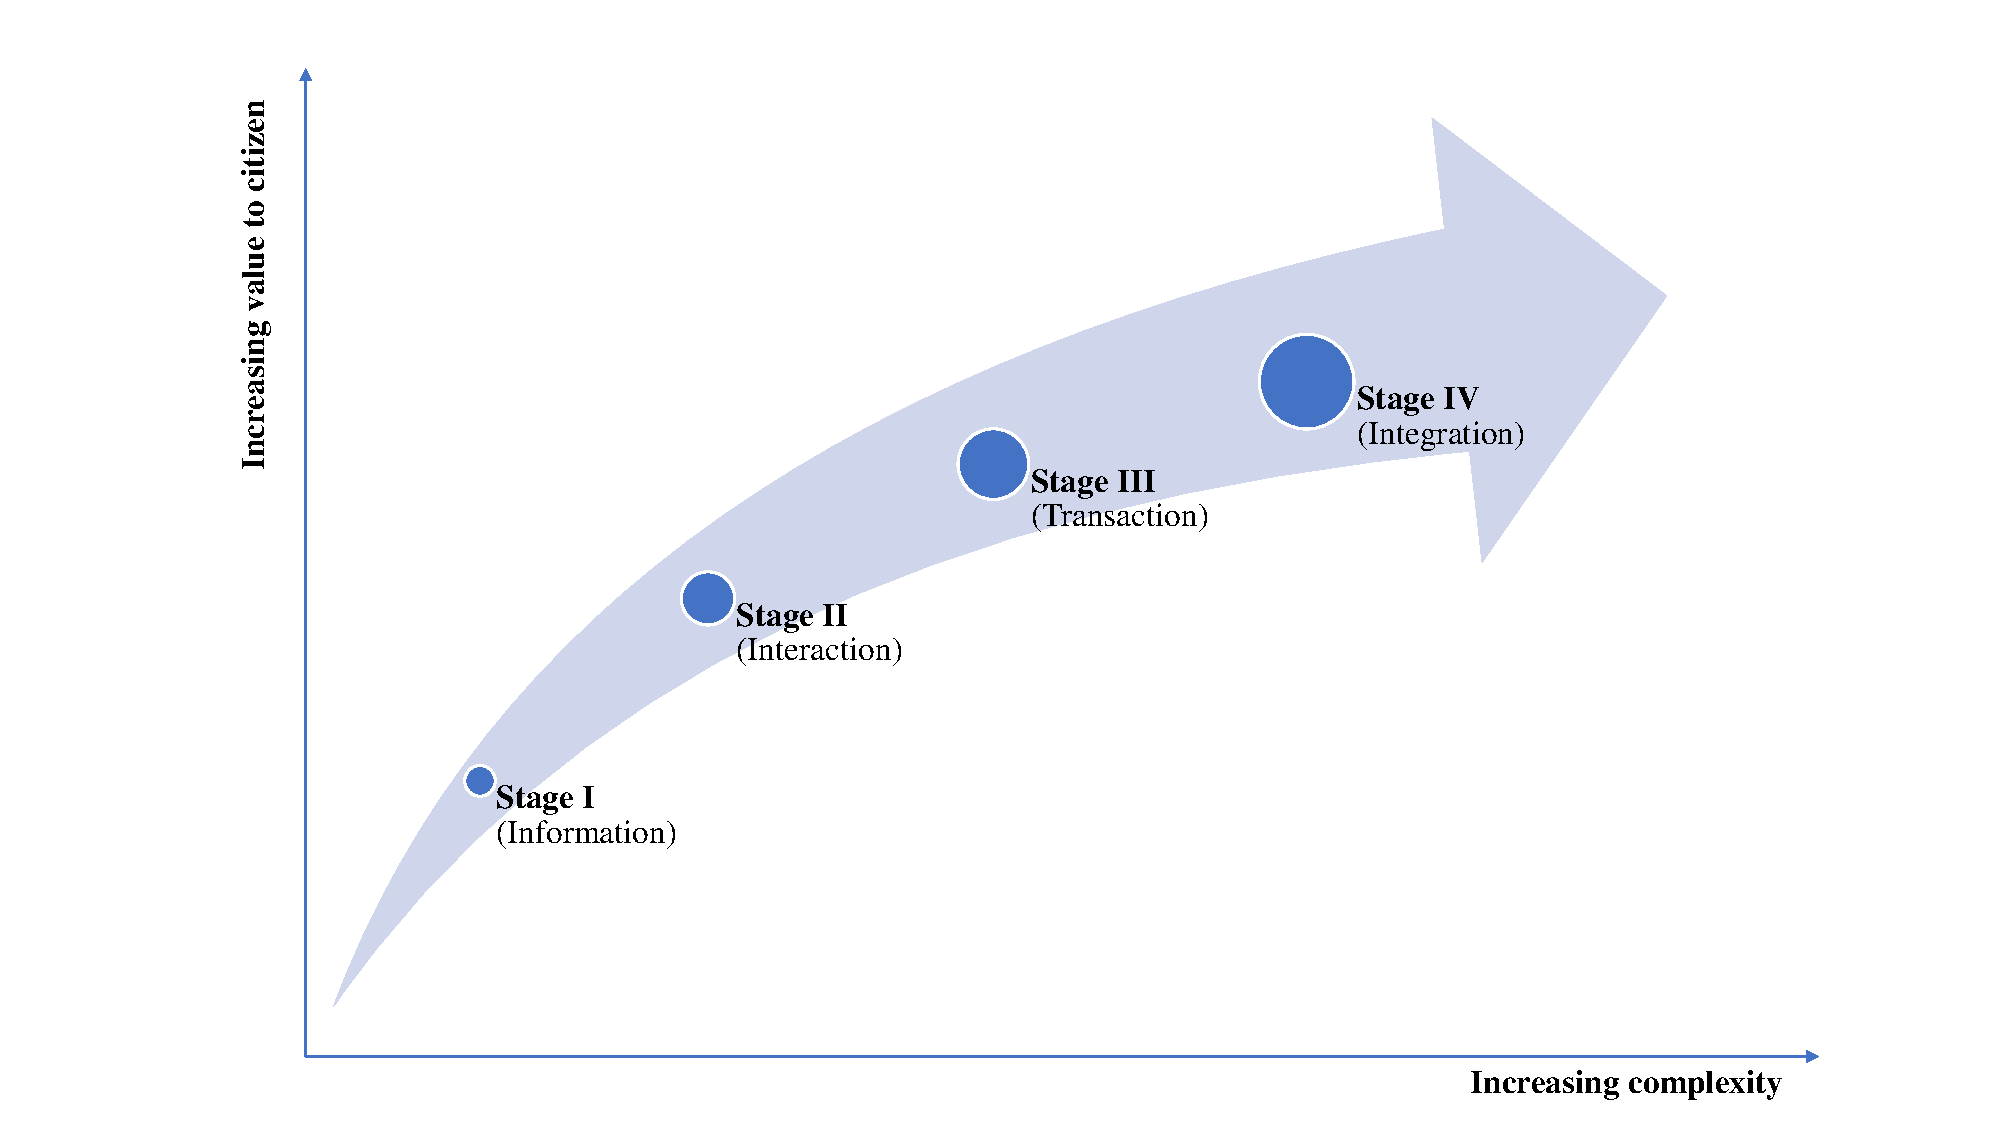
\includegraphics[width=0.9\linewidth]{../Figures/maturity.pdf}
        \caption{4 Phases Maturity Model for e-Governance (\acrshort{un}, ASPA 2002)}
        \label{fig:maturity}
    \end{figure}
    \section{e-Governance Evolution in Nepal}
    \subsection{Summarized History}
    In 1916, telecommunication services were first inaugurated, but it wasn't until 1948  that the general public had access to telecommunication services. During the 1971  census, the use of \acrshort{ibm} 1401 was the first recorded use of such technology for governmental services. Similarly by the late 1990s, the government had set up different agreements with local and international \acrshort{ngo}s for the betterment of health services to the citizens. The transition between the late 1990s and the early 2000s was when the foundation of the current \acrshort{ict} services was built. When the entire world was booming towards \acrfull{www}, Nepal too rode the wave and increased its internet penetration to major cities like Kathmandu, Pokhara, Dharan and Biratnagar. The first \acrshort{it} Policy was drafted in 2000  that went under multiple amendments up until IT Policy 2015. \acrfull{ntc} had already started its 2G expansion throughout the nation starting that lasted till the early 2000s. In 2004, Ncell, (then Mero Mobile) started its service in Nepal. Several infrastructures and institutions namely \acrfull{hlcit}, \acrfull{nitc}, \acrfull{moest}, \acrfull{moic}, \acrfull{moga}, and \acrfull{mof} initiated the \acrfull{egmp}. The \acrfull{eta} was a crucial turning point in Nepal for the implementation of e-Governance as we had entered the transactional stage of maturity. Starting in 2006, the internet penetration in Nepal boomed with a massive exponential growth reaching 90\% at the moment. With the expansion of telecommunication services by \acrshort{ntc}, different private \acrfull{isp} also started gaining trust in Nepal. Currently there is a healthy competition in the \acrshort{isp} market with the introduction of \acrfull{ftth} services. The draft of the wireless broadband master plan 2012 was prepared by \acrshort{itu} for the powerful use of broadband generation in Nepal which is by far the strongest strategic planning of e-Governance in Nepal. With the \acrshort{eta} in implementation, banking, e-Commerce and e-Payment services too started gaining proper growth. Governmental and private banks currently must have mobile banking, \acrshort{atm} and \acrfull{abbs} to be trusted. Similarly international payment is also on the rise with international payment gateways finding ways to penetrate to Nepalese customers. \acrshort{it} Policy of 2015, which was revised in 2018 is a crucial policy for the growth of \acrshort{it} in Nepal. Digital Nepal Framework 2019 is the latest such documentation in Nepal.
    \begin{figure}[H]
        \centering
        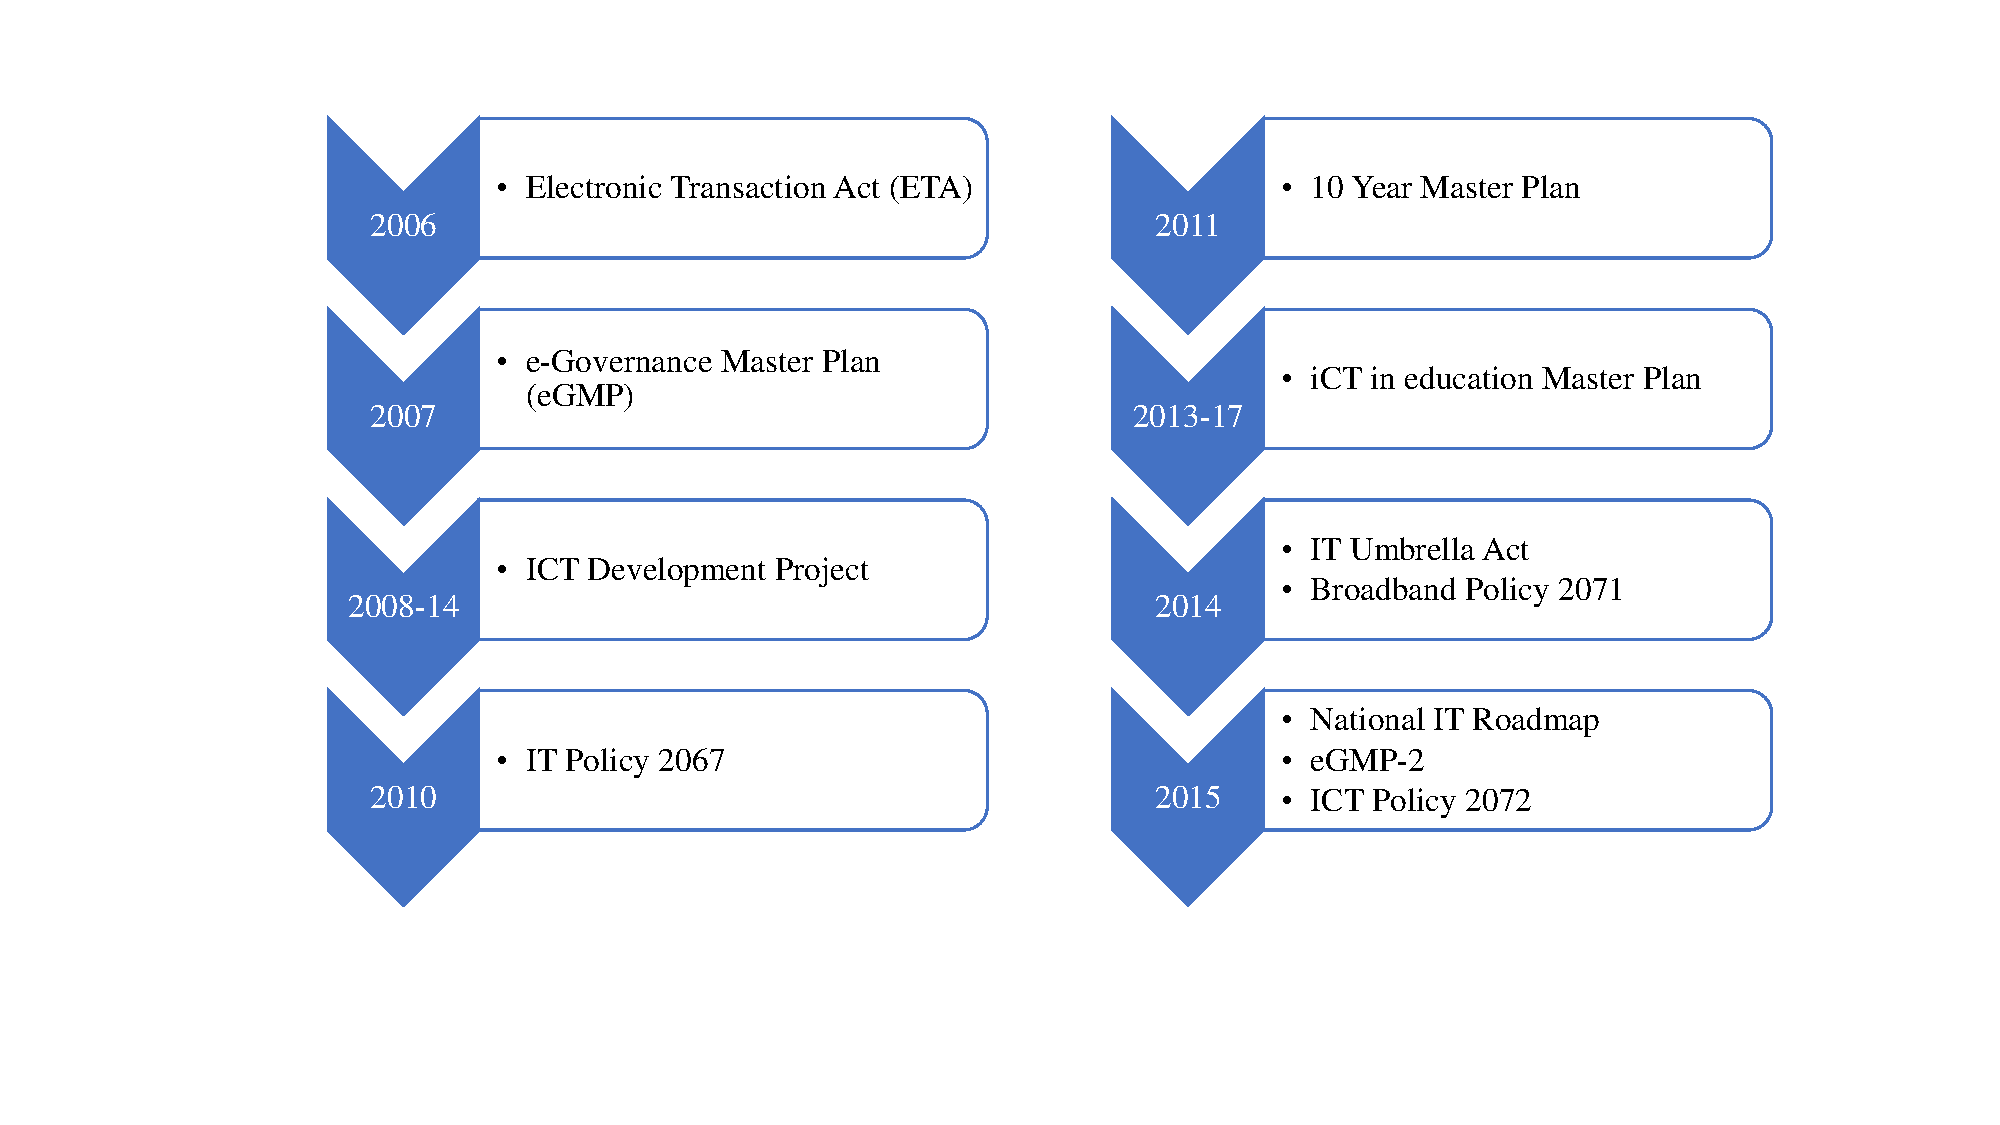
\includegraphics[width=0.9\linewidth]{../Figures/policy.pdf}
        \caption{Key Dates for the \acrshort{it} Policies in Nepal}
        \label{fig:policy}
    \end{figure}
    \subsection{e-Readiness Status}
    e-Readiness refers to a country's ability to take advantage of the internet as an engine of economic growth and human development. Nepal jumped from 135 to 117 rank from 2016 to 2018 with an \acrshort{egdi} score of 0.4748 in 2018. This indicates that Nepal's e-Readiness indicator is headed in the right direction and the country is getting better in utilizing \acrshort{ict} resources.  
    \begin{figure}[H]
        \centering
        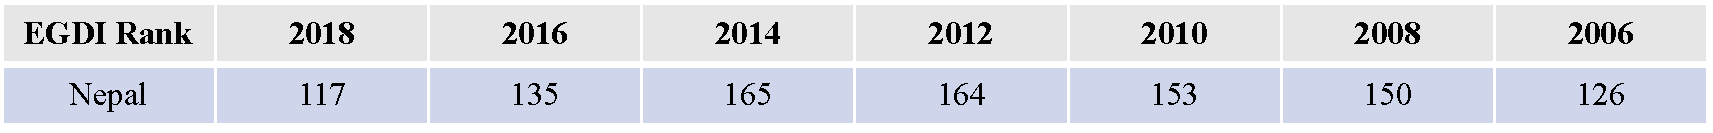
\includegraphics[width=\linewidth]{../Figures/egdi.pdf}
        \caption{\acrfull{egdi} rank of Nepal over the years}
        \label{fig:egdi}
    \end{figure}
    \subsection{e-Governance Status-Quo}
    As indicated by the improved \acrshort{egdi} rank, Nepal's e-Governance status-quo is in the upward trend. With the advent of newer \acrshort{isp}, affordable and faster internet service is on the rise. e-Payment, mobile banking and online transaction services are getting more recognition among the public, and are in the upward trend as well. \Myciteauthor{gajendra2020} points out the status of digital governance in Nepal. The paper elaborates how the current situation due to the \acrshort{covid} pandemic has led some of the organization to have developed their own \acrshort{it} infrastructure and facilitate online learning, online shopping and information sharing. Although initially launched on December 21, 2019, the stable release of the \textit{Nagarik App} on May 2, 2021 has proven to be a game changer in e-Governance status-quo. The application is still evolving and currently provides services related to \acrfull{pan} card, vehicle tax enquiry (payment not included yet), land revenue, police report clearance, educational certificate, personal identification, \textit{Hello Sarkar} complaint. With the entire world moving towards cloud computing via service providers like \acrfull{aws}, \acrfull{gcp} and Microsoft Azure, companies based in Nepal too are adopting cloud infrastructures in their business architectures. \Myciteauthor{giri-cloud} mentions the different existing data security issues in cloud computing and reasons behind such issues. It concludes that Nepal, being a developing country should start using its own server and satellite, which would be a great kickstart for the much needed e-Governance boost. \acrfull{gea} proposed for \acrshort{hlcit} is a cloud architecture that would result in a convenient, transparent and effective e-Governance model for Nepal. 
    \clearpage
    \printbibliography[heading=bibintoc,title={Bibliography}]
\end{document}